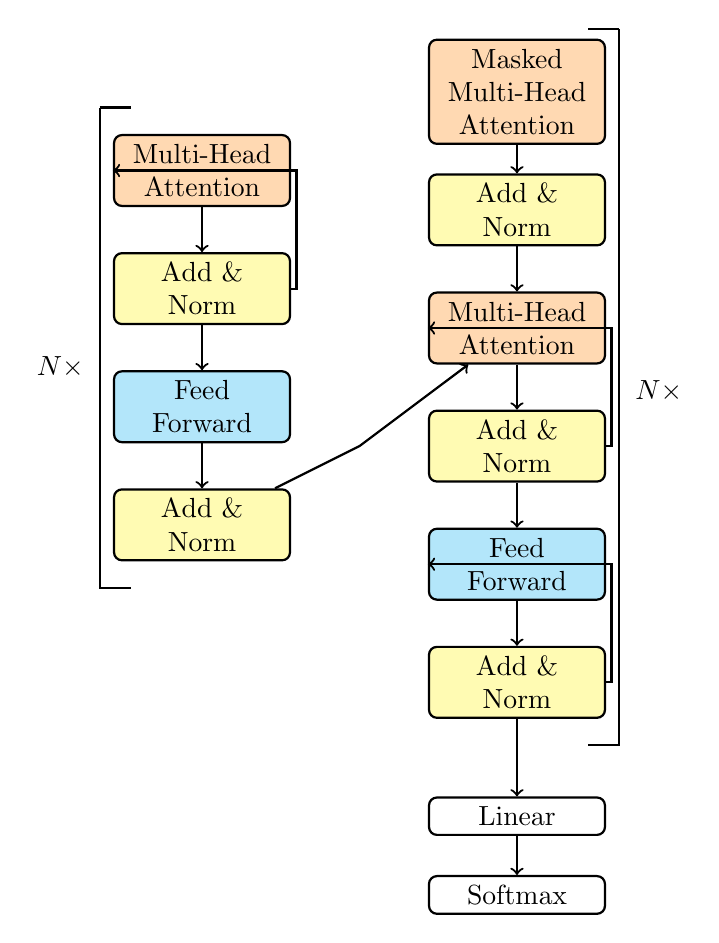
\begin{tikzpicture}[node distance=1.5cm, auto, thick]
  % Define styles
  \tikzstyle{block} = [rectangle, draw, fill=white, text width=2cm, text centered, rounded corners=0.1cm]
  \tikzstyle{attention} = [rectangle, draw, fill=orange!30, text width=2cm, text centered, rounded corners=0.1cm]
  \tikzstyle{norm} = [rectangle, draw, fill=yellow!30, text width=2cm, text centered, rounded corners=0.1cm]
  \tikzstyle{ffwd} = [rectangle, draw, fill=cyan!30, text width=2cm, text centered, rounded corners=0.1cm]
  \tikzstyle{output} = [rectangle, draw, fill=white, text width=2cm, text centered, rounded corners=0.1cm]
  
  % Encoder stack (left side)
  \node[attention] (enc_attn) at (0, 4) {Multi-Head\\Attention};
  \node[norm] (enc_norm1) at (0, 2.5) {Add \& Norm};
  \node[ffwd] (enc_ffwd) at (0, 1) {Feed\\Forward};
  \node[norm] (enc_norm2) at (0, -0.5) {Add \& Norm};
  
  % Encoder bracket
  \draw[thick] (-1.3, 4.8) -- (-1.3, -1.3) -- (-0.9, -1.3);
  \draw[thick] (-1.3, 4.8) -- (-0.9, 4.8);
  \node at (-1.8, 1.5) {$N\times$};
  
  % Decoder stack (right side)
  \node[attention] (dec_masked) at (4, 5) {Masked\\Multi-Head\\Attention};
  \node[norm] (dec_norm1) at (4, 3.5) {Add \& Norm};
  \node[attention] (dec_attn) at (4, 2) {Multi-Head\\Attention};
  \node[norm] (dec_norm2) at (4, 0.5) {Add \& Norm};
  \node[ffwd] (dec_ffwd) at (4, -1) {Feed\\Forward};
  \node[norm] (dec_norm3) at (4, -2.5) {Add \& Norm};
  
  % Decoder bracket
  \draw[thick] (5.3, 5.8) -- (5.3, -3.3) -- (4.9, -3.3);
  \draw[thick] (5.3, 5.8) -- (4.9, 5.8);
  \node at (5.8, 1.2) {$N\times$};
  
  % Output layers
  \node[output] (linear) at (4, -4.2) {Linear};
  \node[output] (softmax) at (4, -5.2) {Softmax};
  
  % Encoder connections
  \draw[->] (enc_attn) -- (enc_norm1);
  \draw[->] (enc_norm1) -- (enc_ffwd);
  \draw[->] (enc_ffwd) -- (enc_norm2);
  
  % Decoder connections
  \draw[->] (dec_masked) -- (dec_norm1);
  \draw[->] (dec_norm1) -- (dec_attn);
  \draw[->] (dec_attn) -- (dec_norm2);
  \draw[->] (dec_norm2) -- (dec_ffwd);
  \draw[->] (dec_ffwd) -- (dec_norm3);
  \draw[->] (dec_norm3) -- (linear);
  \draw[->] (linear) -- (softmax);
  
  % Cross connections from encoder to decoder
  \draw[->] (enc_norm2) -- (2, 0.5) -- (dec_attn);
  
  % Feedback loops (simplified)
  \draw[->] (enc_norm1.east) -- (1.2, 2.5) -- (1.2, 4) -- (enc_attn.west);
  \draw[->] (dec_norm2.east) -- (5.2, 0.5) -- (5.2, 2) -- (dec_attn.west);
  \draw[->] (dec_norm3.east) -- (5.2, -2.5) -- (5.2, -1) -- (dec_ffwd.west);
\end{tikzpicture}